%--------------------------------------------------
\begin{frame}
\frametitle{Encryption for connexions : SSL/TLS}
\begin{itemize}
\item Session layer based, affect application layer (TFP, HTTP, SMTP, IMAP, POP
, DNS, RTMP ...)
\item Prefer using TLS over SSL when you have choice.
\item Asymetrical encryption, forward secrecy (Diffie-Hellman).
\end{itemize}

Only use up to date browser in order to have the correct fingerprint caught
on your computer and avoid MITM attack.
If your browser does not have a certificate pinning system install
certificate patrol (assuming your first connection is safe) or HTTPS everywhere
with the SSL observatory ON.
\end{frame}

\begin{frame}
\frametitle{Diffie-Hellman key exchange}
\begin{columns}[c]
\column{.6\textwidth}
\begin{block}{With color}
\begin{itemize}
\item two people that never met agrees on the same keys
\item heavy use of one-way function
\item Select a public color, then each part select a private secret one.
\item each part mix private/public key and send it to the other.
\item Each part mix the mixture of the other with their own private color and
arrive to the same final private color.
\end{itemize}
\end{block}
\column{.4\textwidth}
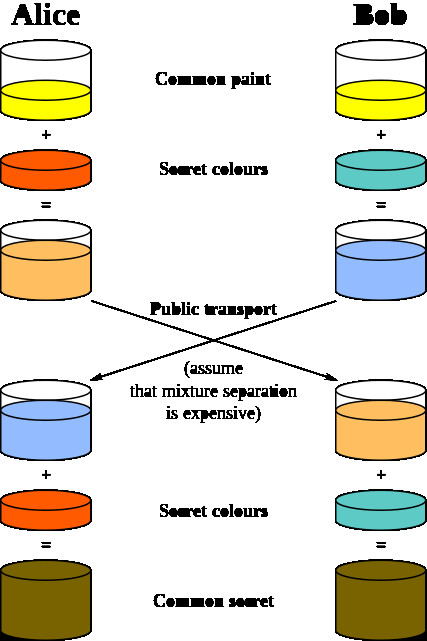
\includegraphics[height=.8\textheight]{./materials/diffie-hellman}
\end{columns}
\end{frame}
%----------------------------------------------------
\begin{frame}
\frametitle{Diffie-Hellman key exchange}
\begin{columns}[c]
\column{.6\textwidth}
\begin{block}{With maths : (modular|clock) arithmetic}
\begin{itemize}
\item work on prime modulus and generator of that modulus.
\item $3^n mod 17 = X$ with $0 <= X <= 17$ hard to reverse when len(prime modulus)
increase.
\item so each part agrees on a prime modulus (p) and a generator (g).
Then calculate $g^{secret} mod(p)=Mix$ and send it publicly.
\item each part compute now $Mix^{secret} mod(p)=Key$
\end{itemize}
\end{block}
\column{.4\textwidth}
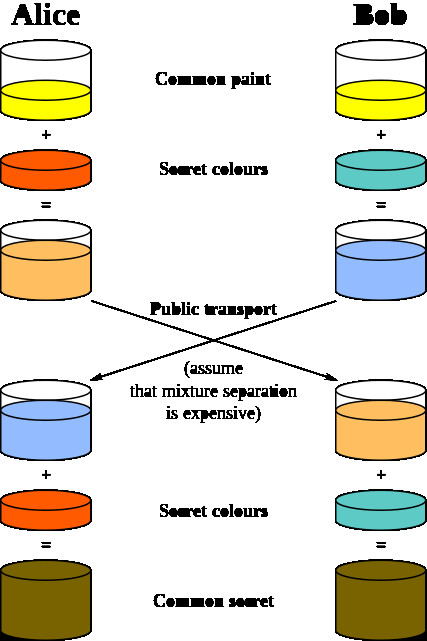
\includegraphics[height=.8\textheight]{./materials/diffie-hellman}
\end{columns}
\end{frame}
%--------------------------------------------------
\begin{frame}
\frametitle{Encryption for chat sessions : OTR}
\begin{block}{OTR : Off-the-Record Messaging}
\begin{itemize}
\item Diffie-Hellman key exchange
\item off-the-record conversation
\item repudiable authentication by using message authentication codes.
\\(authentication ON | digital signature OFF)
\end{itemize}
\end{block}
Bob cannot prove that Alice generated the MAC.
Install Pidgin (cross-plateform) with plugin (available from the OTR homepage)
and start playing.
\end{frame}
%----------------------------------------------------
\begin{frame}
\frametitle{Encryption for disk}
Many possibilities, but full disk encryption is advised in case you really care
about privacy. For this purpose you have a plethora of choice.
\begin{itemize}
\item Stacked filesystem encryption (eCryptfs, EncFs, disk utility ...)
\item Disk encryption (dm-crypt, GELI, FileVault, DiskCryptor, trueCrypt ...)
\end{itemize}
\begin{block}{Case study : Plain dm-crypt}
\begin{itemize}
\item full disk encryption
\item bootloader and key on external device
\end{itemize}
\end{block}
(can also be done with Diskcryptor)
\end{frame}
%----------------------------------------------------
\begin{frame}
\frametitle{Encryption for smartphone}
\begin{block}{Android}
\begin{itemize}
\item Chatsecure (Facebook chat, GTalk, Jabber) [OTR Messaging]
\item Textsecure (SMS)
\item LUKS Manager (ROOT requiered)
\end{itemize}
\end{block}
\begin{block}{iOS}
\begin{itemize}
\item Chatsecure (Facebook chat, GTalk, Jabber) [OTR Messaging]
\item FDE available by default, bypass techniques available, proprietary
built system...\\ (More details : iPhone Forensic, O'Reilly)
\end{itemize}
\end{block}
\end{frame}
%----------------------------------------------------
\begin{frame}
\frametitle{Example:  chatsecure with facebook}
\begin{columns}[c]
    \column{.5\textwidth}
    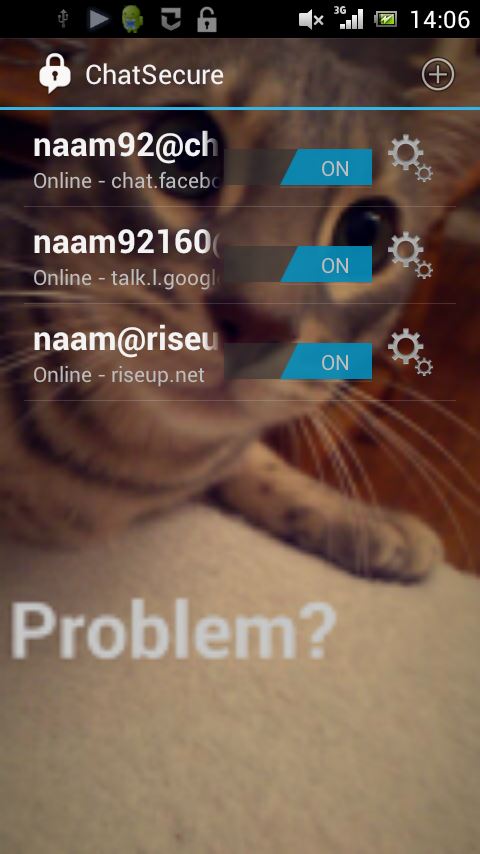
\includegraphics[height=.9\textheight]{./materials/chat_secure_account}
    \column{.5\textwidth}
    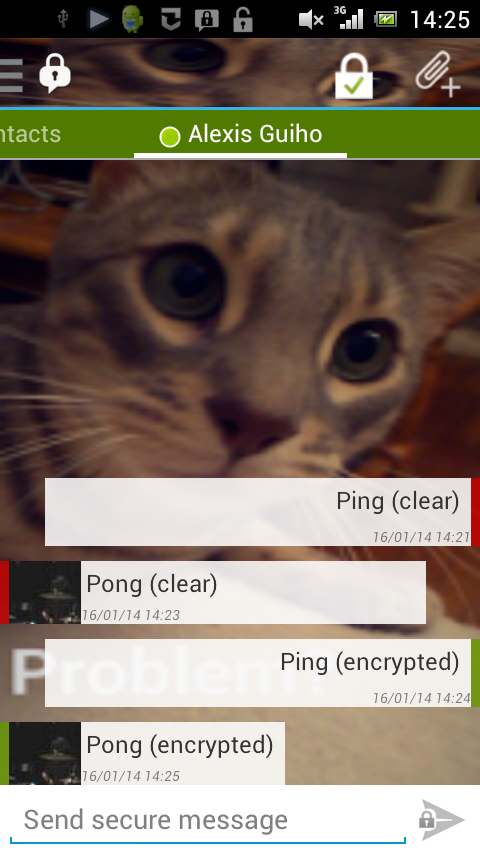
\includegraphics[height=.9\textheight]{./materials/chat_secure_conv}
\end{columns}
\end{frame}
%----------------------------------------------------
\begin{frame}
    \frametitle{Example : chatsecure with facebook}
    \begin{columns}[c]
    \column{.5\textwidth}
    Win.
    \begin{itemize}
    \item Facebook cannot read your messages.
    \item But you can't read it anymore after your current session.
    \end{itemize}
    \column{.5\textwidth}
    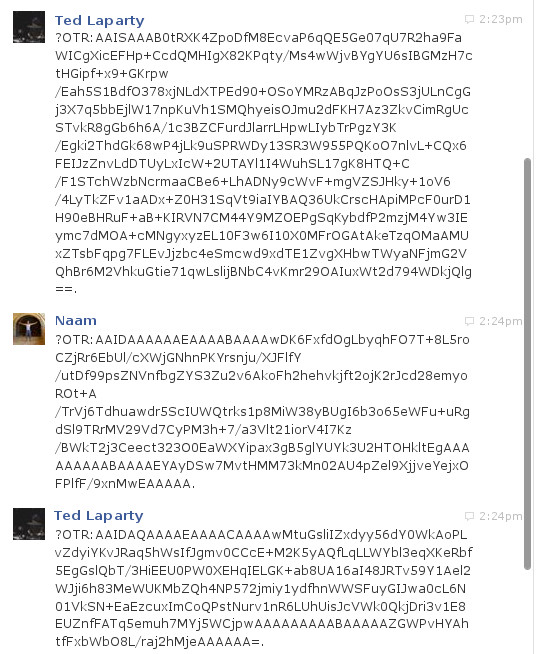
\includegraphics[height=.9\textheight]{./materials/fb_otr}
    \end{columns}
\end{frame}
\begin{frame}
\frametitle{Encryption for files}
\begin{block}{Mails : Use GPG}
\begin{itemize}
\item create your keys
\item share your public key
\item enter the \sout{matrix} Web Of Trust (WOT)
\item encrypt/sign your message and send it.
\item receive mails too.
\end{itemize}
\end{block}
\begin{block}{Files}
Basically you can do the same with 'regular file'...
Make sure not to store keys near encrypted files, prefer symetrical encryption
if files will not be shared.
\end{block}
\end{frame}

%----------------------------------------------------
\begin{frame}
\frametitle{Choosing a password : Diceware method}
The diceware method allow you to construct very strong password with the
following advantages :
\begin{itemize}
\item Very easy to remember
\item strong passphrase with high entropy (~20char +)
\item truly random; password is totally detached from user habits/knowledge
etc.
\end{itemize}
\begin{block}{Test your password strength in bits}
Entropy calculated by : $H_{tn}=\sum_{k=1}^nL*\frac{Log N}{Log 2}$
\end{block}
Do \emph{NOT} test your password strength online.
Take a calculator and calcul the entropy yourself.
\end{frame}
%----------------------------------------------------
\begin{frame}
\frametitle{Diceware, overall strength}
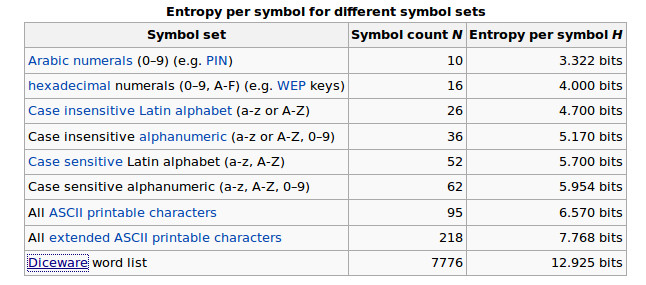
\includegraphics[width=0.8\linewidth]{./materials/diceware}
\end{frame}
%----------------------------------------------------
\begin{frame}
\frametitle{Diceware, how does it work}
You only need a true random source and an official mapped dictionary. \\
\begin{columns}[c]
\column{.5\textwidth}
\begin{itemize}
\item Draw 1 : 5 1 5 5 5
\item Draw 2 : 5 4 5 6 6
\item Draw 3 : 6 5 6 4 6
\item Draw 4 : 5 4 3 1 2
\item Draw 5 : 2 2 3 5 4
\end{itemize}
\column{.5\textwidth}
\begin{itemize}
\item ...
\item 14245 bit
\item 14246 bitch
\item 14247 bite
\item ...
\end{itemize}
\end{columns}
\begin{block}{Results}
\begin{itemize}
\item in French : phase ribose vv rebut clebs
\item in English : rest sober 80 skye data
\end{itemize}
\end{block}
\end{frame}
